\documentclass[12pt]{article}
\usepackage{amsmath}
\usepackage{graphicx}
\usepackage{hyperref}
\usepackage{listings}
\usepackage{color}
\usepackage{pythonhighlight}
\usepackage{caption}

\title{Operating System Course Report - First Half of the Semester}
\author{A class}
\date{\today}

\begin{document}

\maketitle
\newpage

\tableofcontents
\newpage

\section{Introduction}
This report summarizes the topics covered during the first half of the Operating System course. It includes theoretical concepts, practical implementations, and assignments. The course focuses on the fundamentals of operating systems, including system architecture, process management, CPU scheduling, and deadlock handling.

\section{Course Overview}
\subsection{Objectives}
The main objectives of this course are:
\begin{itemize}
    \item To understand the basic components and architecture of a computer system.
    \item To learn process management, scheduling, and inter-process communication.
    \item To explore file systems, input/output management, and virtualization.
    \item To study the prevention and handling of deadlocks in operating systems.
\end{itemize}

\subsection{Course Structure}
The course is divided into two halves. This report focuses on the first half, which covers:
\begin{itemize}
    \item Basic Concepts and Components of Computer Systems
    \item System Performance and Metrics
    \item System Architecture of Computer Systems
    \item Process Description and Control
    \item Scheduling Algorithms
    \item Process Creation and Termination
    \item Introduction to Threads
    \item File Systems
    \item Input and Output Management
    \item Deadlock Introduction and Prevention
    \item User Interface Management
    \item Virtualization in Operating Systems
\end{itemize}

\section{Topics Covered}

\subsection{Basic Concepts and Components of Computer Systems}
This section explains the fundamental components that make up a computer system, including the CPU, memory, storage, and input/output devices.

\subsection{System Performance and Metrics}
This section introduces various system performance metrics used to measure the efficiency of a computer system, including throughput, response time, and utilization.

\subsection{System Architecture of Computer Systems}
Describes the architecture of modern computer systems, focusing on the interaction between hardware and the operating system.

\subsection{Process Description and Control}
Processes are a central concept in operating systems. This section covers:
\begin{itemize}
    \item Process states and state transitions
    \item Process control block (PCB)
    \item Context switching
\end{itemize}

\subsection{Scheduling Algorithms}
This section covers:
\begin{itemize}
    \item First-Come, First-Served (FCFS)
    \item Shortest Job Next (SJN)
    \item Round Robin (RR)
\end{itemize}
It explains how these algorithms are used to allocate CPU time to processes.

\subsection{Process Creation and Termination}
Details how processes are created and terminated by the operating system, including:
\begin{itemize}
    \item Process spawning
    \item Process termination conditions
\end{itemize}

\subsection{Introduction to Threads}
This section introduces the concept of threads and their relation to processes, covering:
\begin{itemize}
    \item Single-threaded vs. multi-threaded processes
    \item Benefits of multithreading
\end{itemize}

% \begin{figure}[h]
%     \centering
%     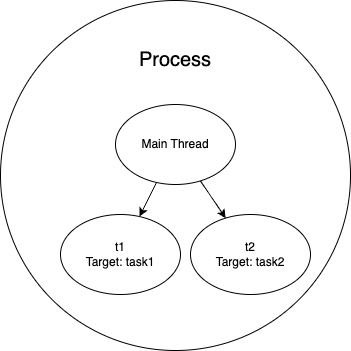
\includegraphics[width=0.5\textwidth]{/Users/khawaritzmi/Unhas/os_report_mid2024/a_class/asset/example.png}  % Sesuaikan nama file dan ukurannya
%     \caption{Ini adalah gambar contoh dari multithreading.}
%     \label{fig:contoh_gambar}
% \end{figure}

% Seperti yang terlihat pada Gambar \ref{fig:contoh_gambar}, inilah cara menambahkan gambar dengan keterangan.

\subsection{File Systems}
File systems provide a way for the operating system to store, retrieve, and manage data. This section explains:
\begin{itemize}
    \item File system structure
    \item File access methods
    \item Directory management
\end{itemize}

\subsection{Input and Output Management}
Input and output management is key for handling the interaction between the system and external devices. This section includes:

\subsubsection{Struktur \textit{Input/Output}}
\begin{figure}[h] % [h] artinya gambar diletakkan 'here' (di sini)
    \centering
    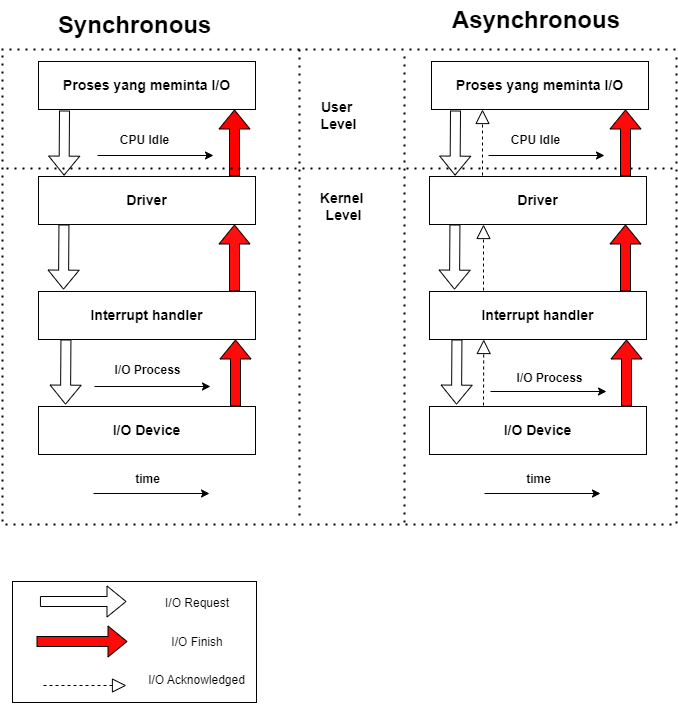
\includegraphics[width=0.5\textwidth]{asset/Struktur_IO.png}
    \captionsetup{labelformat=empty}
    \caption{Gambar 1 : Struktur I/O \emph{Synchronous} dan \emph{Asynchronous.}}
    \label{Gambar 1}
\end{figure}

Nurasyifa, dkk (2024) menjelaskan bahwa struktur I/O terbagi menjadi dua yaitu:
\begin{enumerate}
    \item Struktur I/O \emph{Synchronous} 
    \begin{enumerate}
        \item Karakteristik :
        \begin{itemize}
            \item Proses yang meminta I/O akan menunggu hingga operasi I/O selesai.
            \item CPU akan \emph{idle} (tidak melakukan pekerjaan lain) selama menunggu operasi I/O.
        \end{itemize}
        \item Alur Kerja:
        \begin{itemize}
            \item Proses aplikasi \emph{user level} meminta operasi I/O.
            \item Permintaan diteruskan ke \textit{driver} perangkat.
            \item \textit{Driver} akan melakukan operasi I/O dan menunggu hingga selesai.
            \item Setelah selesai, \textit{driver} akan memberitahu proses aplikasi.
            \item Proses aplikasi kemudian dapat melanjutkan pekerjaannya.
        \end{itemize}
        \item Kelebihan: Sederhana untuk diimplementasikan.
        \item Kekurangan:
        \begin{itemize}
            \item Efisiensi CPU rendah karena CPU harus menunggu.
            \item Respons sistem menjadi lambat, terutama untuk operasi I/O yang lama.    
        \end{itemize}
    \end{enumerate}

    \item Struktur I/O \emph{Asynchronous}
    \begin{enumerate}
        \item Karakteristik
        \begin{itemize}
            \item Proses yang meminta I/O tidak perlu menunggu, melainkan dapat melanjutkan pekerjaan lain.
            \item CPU dapat melakukan tugas lain selama operasi I/O berlangsung.  
        \end{itemize}

        \item Alur Kerja:
        \begin{itemize}
            \item Proses aplikasi meminta operasi I/O.
            \item Permintaan diteruskan ke \textit{driver} perangkat.
            \item \textit{Driver} akan memulai operasi I/O dan memberikan kendali kembali ke CPU.
            \item Saat operasi I/O selesai, perangkat akan mengirimkan interupsi ke CPU.
            \item CPU akan merespons interupsi dengan menjalankan \emph{interrupt handler.}
            \item \emph{Interrupt handler} akan memberitahu proses aplikasi bahwa operasi I/O telah selesai. 
        \end{itemize}

        \item Kelebihan
        \begin{itemize}
            \item Efisiensi CPU tinggi karena CPU dapat melakukan tugas lain.
            \item Respons sistem lebih cepat.
        \end{itemize}

        \item Kekurangan:
        \begin{itemize}
            \item Implementasinya lebih kompleks
            \item Membutuhkan mekanisme penanganan interupsi
        \end{itemize}
    \end{enumerate}
\end{enumerate}

\subsubsection{Metode Operasi Sistem \textit{Input/Output}}
\begin{enumerate}
    \item I/O Terprogram \par
    Metode ini melibatkan CPU secara langsung dalam proses pengiriman dan penerimaan data dari perangkat I/O. Dalam I/O terprogram, CPU harus memeriksa secara terus-menerus \textit{(polling)} apakah perangkat I/O siap untuk melakukan transfer data. CPU kemudian mentransfer data secara manual antara perangkat dan memori. Ini menyebabkan CPU terlibat penuh dalam operasi I/O dan tidak dapat melakukan tugas lain selama proses berlangsung. Salah satu kelemahan utama metode ini adalah efisiensinya yang rendah karena CPU harus menunggu perangkat I/O untuk siap.
    
    \item I/O \emph{Interrupt Driven} \par
    Pada metode ini, perangkat I/O mengirim sinyal interupsi kepada CPU ketika perangkat tersebut siap untuk menerima atau mengirim data. CPU tidak perlu terus-menerus memeriksa status perangkat I/O, sehingga bisa mengerjakan tugas lain sampai menerima interupsi. Ketika interupsi terjadi, CPU menghentikan sementara tugas yang sedang dilakukan, menangani interupsi untuk menyelesaikan operasi I/O, kemudian kembali melanjutkan tugas sebelumnya. Metode ini lebih efisien dibandingkan I/O terprogram karena CPU tidak selalu terikat dengan perangkat I/O dan bisa mengerjakan tugas lain sambil menunggu interupsi.
    
    \item \emph{Direct Memory Access} (DMA) \par
    DMA adalah metode yang memungkinkan perangkat I/O mengakses memori secara langsung tanpa melibatkan CPU dalam proses transfer data. Dengan menggunakan DMA \emph{controller}, data dapat ditransfer antara perangkat I/O dan memori secara mandiri, sementara CPU hanya diberi tahu ketika operasi transfer selesai. Metode ini sangat efisien karena memungkinkan CPU untuk melakukan tugas lain tanpa harus terlibat langsung dalam proses I/O, sehingga cocok untuk transfer data dalam jumlah besar atau operasi I/O yang intensif.
\end{enumerate}

\subsubsection{\emph{Interrupt Handler}}
Apabila suatu transfer selesai maka pengontrol biasanya menyebabkan suatu \textit{interupt} yang memaksa CPU untuk menunda menjalankan programnya dan mulai menjalankan prosedur khusus yang disebut \emph{interupt handler}. \emph{Interupt handler} adalah kondisi dimana CPU menunda program yang sedang dijalankan dan berganti menjalankan program khusus pada saat akses memori langsung sedang berlangsung dan minta \emph{interupt}.

\begin{thebibliography}{10}
    \bibitem{Jurnal Kendali Teknik dan Sains}
    Alifah, N., Deanda, G. V., Juniwan, Aribowo, D. (2023).Peran Teknologi Input dan Output dalam Pengembangan Perangkat Keras.\textit{Jurnal Kendali Teknik dan Sains,}.1(4), 123-136.

    \bibitem{builtin}
    Gallo, K. (2024,September20). \textit{builtin.} Retrieved from https://builtin.com/hardware/i-o-input-output
    
    \bibitem{Jurnal Multidisiplin Saintek}
    Nurasyifa, N., Sheril, J. A., Maulana, M. R., Muiz, A.,Febrian.(2024). ANALISIS INPUT/OUTPUT:PERANGKAT DAN INTERFACE PADA ORGANISASI ARSITEKTUR KOMPUTER.\textit{Jurnal Multidisiplin Saintek,} 3(6), 100-111.

\end{thebibliography}

\pagebreak

\subsection{Deadlock Introduction and Prevention}
Explores the concept of deadlocks and methods for preventing them:
\begin{itemize}
    \item Deadlock conditions
    \item Deadlock prevention techniques
\end{itemize}

\subsection{User Interface Management}
This section discusses the role of the operating system in managing the user interface. Topics covered include:
\begin{itemize}
    \item Graphical User Interface (GUI)
    \item Command-Line Interface (CLI)
    \item Interaction between the user and the operating system
\end{itemize}

\subsection{Virtualization in Operating Systems}
Virtualization allows multiple operating systems to run concurrently on a single physical machine. This section explores:
\begin{itemize}
    \item Concept of virtualization
    \item Hypervisors and their types
    \item Benefits of virtualization in modern computing
\end{itemize}

\section{Assignments and Practical Work}
\subsection{Assignment 1: Process Scheduling}
Students were tasked with implementing various process scheduling algorithms (e.g., FCFS, SJN, and RR) and comparing their performance under different conditions.
\subsubsection{Group 1}
\begin{python}
    class Process:
    def __init__(self, pid, arrival_time, burst_time):
        self.pid = pid
        self.arrival_time = arrival_time
        self.burst_time = burst_time
        self.completion_time = 0
        self.turnaround_time = 0
        self.waiting_time = 0
\end{python}

\begin{table}[htbp] % Optional: For floating position
    \centering
    \begin{tabular}{|c|c|c|} % Defines number of columns and alignment (c = center, l = left, r = right). '|' creates vertical lines.
    \hline
    Header 1 & Header 2 & Header 3 \\ % Column headers
    \hline
    Row 1, Column 1 & Row 1, Column 2 & Row 1, Column 3 \\ % First row of data
    \hline
    Row 2, Column 1 & Row 2, Column 2 & Row 2, Column 3 \\ % Second row of data
    \hline
    \end{tabular}
    \caption{Your table caption} % Optional: For adding a caption
    \label{tab:your_label} % Optional: For cross-referencing the table
\end{table}
\subsection{Assignment 2: Deadlock Handling}
In this assignment, students were asked to simulate different deadlock scenarios and explore various prevention methods.

\subsection{Assignment 3: Multithreading and Amdahl's Law}
This assignment involved designing a multithreading scenario to solve a computationally intensive problem. Students then applied **Amdahl's Law** to calculate the theoretical speedup of the program as the number of threads increased.

\subsection{Assignment 4: Simple Command-Line Interface (CLI) for User Interface Management}
Students were tasked with creating a simple **CLI** for user interface management. The CLI should support basic commands such as file manipulation (creating, listing, and deleting files), process management, and system status reporting.

\subsubsection{Group 9}
\begin{itemize}
    \item \textbf{Tugas Pemrograman CLI : Manajemen Antarmuka Pengguna}
\end{itemize}
\par \textbf{Deskripsi Tugas:} Buatlah sebuah program \textit{Command Line Interface (CLI)} sederhana untuk manajemen antarmuka pengguna. Program ini harus mendukung perintah-perintah dasar berikut:
\begin{enumerate}
    \item Manipulasi berkas baru:
    \begin{itemize}
        \item Membuat Berkas baru
        \item Menampilkan daftar berkas dalam direktori saat ini.
        \item Menghapus berkas yang dipilih.
    \end{itemize}
    \item Manajemen Proses
    \begin{itemize}
        \item Menampilkan daftar proses yang sedang berjalan di sistem.
        \item Menghentikan proses berdasarkan PID \textit{(Process ID)}.
    \end{itemize}
    \item Pelaporan Status Sistem
    \begin{itemize}
        \item Menampilkan penggunaan CPU saat ini.
        \item Menampilkan penggunaan memori saat ini.
        \item Menampilkan waktu aktif sistem \textit{(uptime).}
    \end{itemize}
\end{enumerate}
\par \textbf{Ketentuan :}
\begin{enumerate}
    \item Program harus berjalan di lingkungan CLI \textit{(Command Line Interface)} tanpa antarmuka grafis.
    \item Pengguna dapat memasukkan perintah melalui CLI untuk menjalankan fungsi yang diinginkan.
    \item Buat dokumentasi singkat mengenai cara penggunaan program (petunjuk perintah).
\end{enumerate}
\par \textbf{Fitur Tambahan (Opsional):}
\begin{itemize}
    \item Menyediakan opsi untuk menampilkan daftar direktori saat ini.
    \item Menampilkan informasi jaringan seperti alamat IP atau kecepatan jaringan.
    \item Membuat \textit{log} aktivitas untuk setiap perintah yang dijalankan.
\end{itemize}
\par \textbf{Contoh Perintah CLI yang Diharapkan:}
\begin{itemize}
    \item \textit{create-file} 
    \item \textit{list-files}
    \item \textit{delete-file} 
    \item \textit{list-processes}
    \item \textit{kill-process} 
    \item \textit{cpu-status}
    \item \textit{memory-status}
    \item \textit{system-uptime}
\end{itemize}
\par \textbf{Jawaban:}
\begin{python}
import os
import psutil
import time

def create_file(filename):
    """Membuat file baru."""
    try:
        with open(filename, 'w') as f:
            f.write('')  # Membuat file kosong
        print(f"File '{filename}' berhasil dibuat.")
    except Exception as e:
        print(f"Gagal membuat file: {e}")

def list_files():
    """Menampilkan daftar file di direktori saat ini."""
    files = os.listdir('.')
    print("Daftar berkas:")
    for f in files:
        print(f"- {f}")

def delete_file(filename):
    """Menghapus file."""
    try:
        os.remove(filename)
        print(f"File '{filename}' berhasil dihapus.")
    except Exception as e:
        print(f"Gagal menghapus file: {e}")

def list_processes():
    """Menampilkan daftar proses yang berjalan."""
    processes = psutil.pids()
    for pid in processes:
        p = psutil.Process(pid)
        print(f"PID: {pid}, Name: {p.name()}, Status: {p.status()}")

def kill_process(pid):
    """Menghentikan proses berdasarkan PID."""
    try:
        p = psutil.Process(int(pid))
        p.terminate()
        print(f"Proses dengan PID {pid} berhasil dihentikan.")
    except Exception as e:
        print(f"Gagal menghentikan proses: {e}")

def cpu_status():
    """Menampilkan status penggunaan CPU."""
    cpu_percent = psutil.cpu_percent(interval=1)
    print(f"Penggunaan CPU: {cpu_percent}%")

def memory_status():
    """Menampilkan status penggunaan memori."""
    mem = psutil.virtual_memory()
    print(f"Total Memori: {mem.total // (1024 ** 2)} MB")
    print(f"Memori Terpakai: {mem.used // (1024 ** 2)} MB")
    print(f"Memori Bebas: {mem.available // (1024 ** 2)} MB")

def system_uptime():
    """Menampilkan uptime sistem."""
    uptime_seconds = time.time() - psutil.boot_time()
    uptime_str = time.strftime("%H:%M:%S", time.gmtime(uptime_seconds))
    print(f"System Uptime: {uptime_str}")

def main():
    while True:
        print("\nPerintah CLI yang tersedia:")
        print("1. create-file <nama_berkas>")
        print("2. list-files")
        print("3. delete-file <nama_berkas>")
        print("4. list-processes")
        print("5. kill-process <pid>")
        print("6. cpu-status")
        print("7. memory-status")
        print("8. system-uptime")
        print("9. exit")

        command = input("\nMasukkan perintah: ").split()

        if len(command) == 0:
            continue

        if command[0] == "create-file" and len(command) == 2:
            create_file(command[1])
        elif command[0] == "list-files":
            list_files()
        elif command[0] == "delete-file" and len(command) == 2:
            delete_file(command[1])
        elif command[0] == "list-processes":
            list_processes()
        elif command[0] == "kill-process" and len(command) == 2:
            kill_process(command[1])
        elif command[0] == "cpu-status":
            cpu_status()
        elif command[0] == "memory-status":
            memory_status()
        elif command[0] == "system-uptime":
            system_uptime()
        elif command[0] == "exit":
            print("Keluar dari program.")
            break
        else:
            print("Perintah tidak valid. Coba lagi.")

if __name__ == "__main__":
    main()

\end{python}

\subsection{Assignment 5: File System Access}
In this assignment, students implemented file system access routines, including:
\begin{itemize}
    \item File creation and deletion
    \item Reading from and writing to files
    \item Navigating directories and managing file permissions
\end{itemize}

\section{Conclusion}
The first half of the course introduced core operating system concepts, including process management, scheduling, multithreading, and file system access. These topics provided a foundation for more advanced topics to be covered in the second half of the course.

\end{document}

